\documentclass[12pt]{article}

\usepackage{tikz}
\usepackage[simplified]{pgf-umlcd}

\usepackage[landscape]{geometry}
\geometry{left=.5in, right=.5in}

\begin{document}
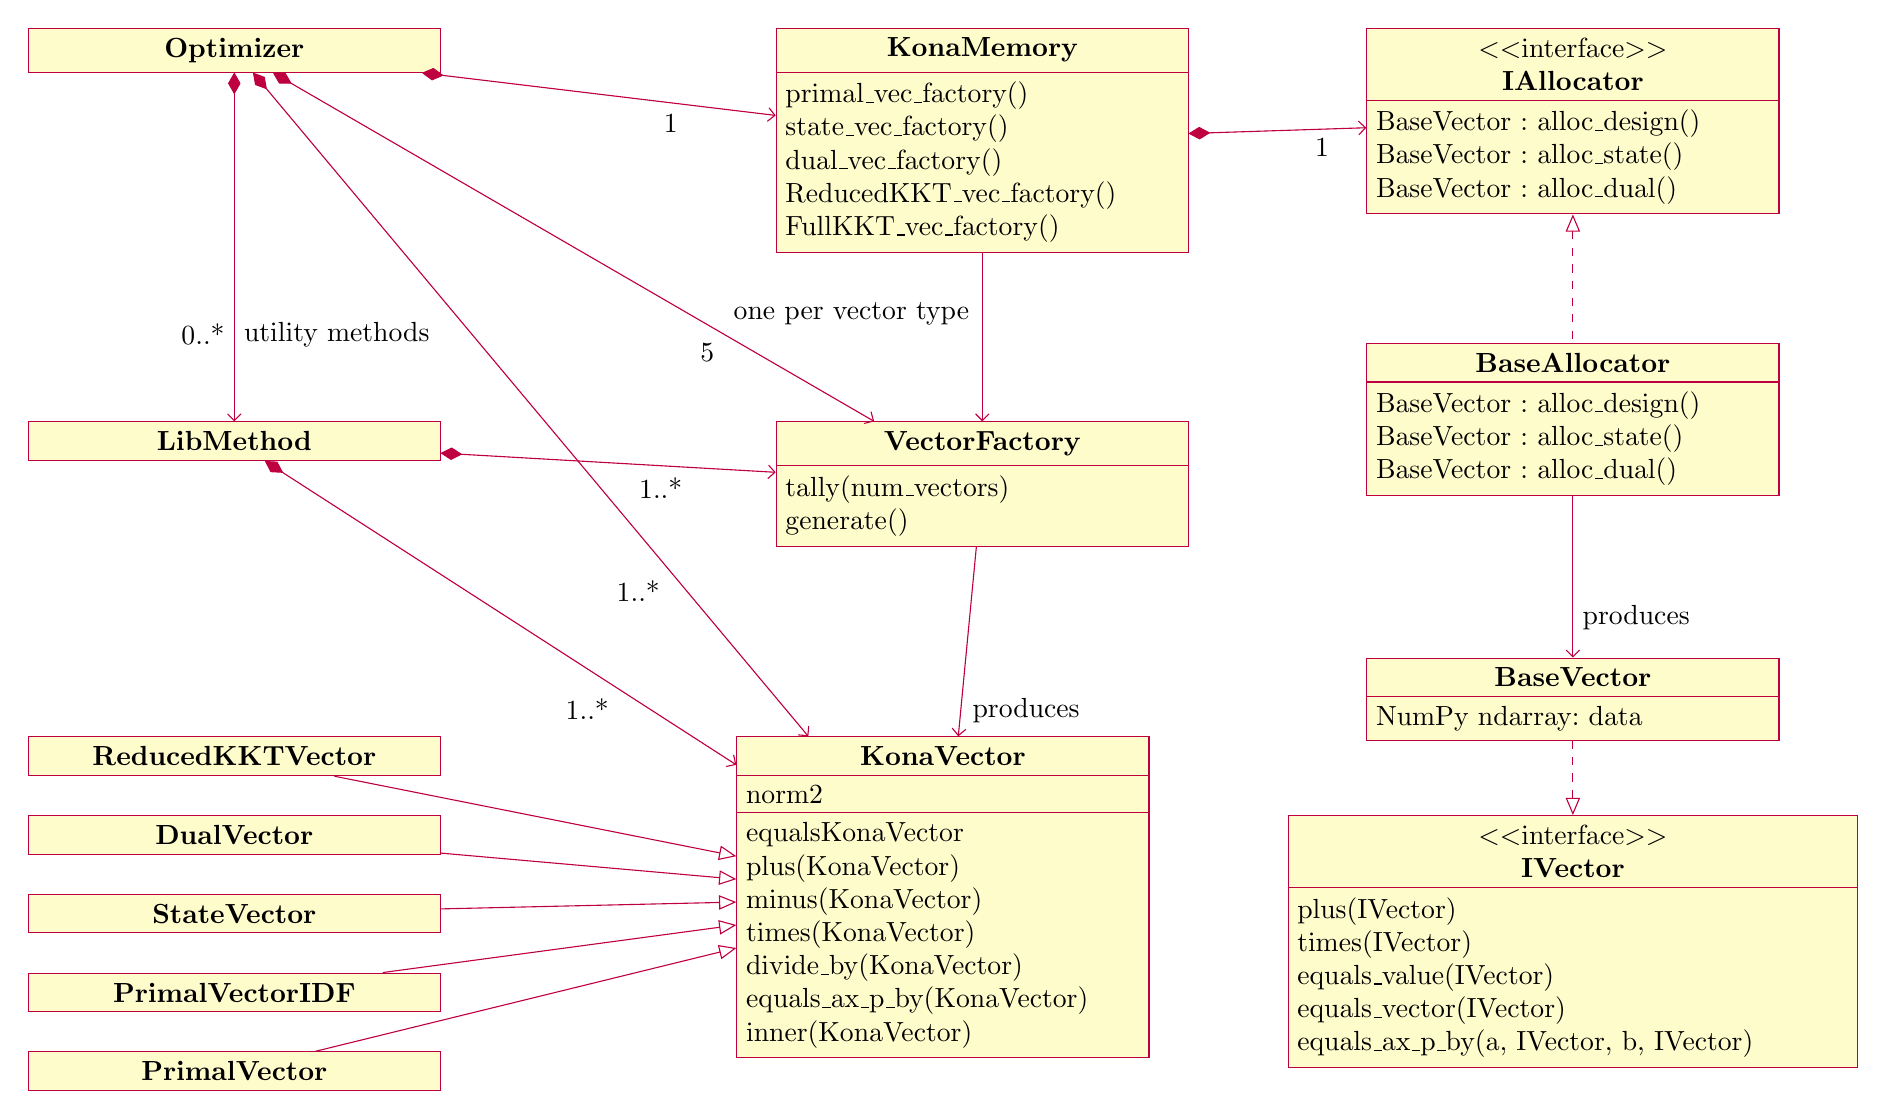
\begin{tikzpicture}[]% [ show background grid ]
    \begin{interface}[text width =7cm ]{IVector}{17,0}
        \operation{plus(IVector)}
        \operation{times(IVector)}
        \operation{equals\_value(IVector)}
        \operation{equals\_vector(IVector)}
        \operation{equals\_ax\_p\_by(a, IVector, b, IVector)}
    \end{interface}

    \begin{interface}{IAllocator}{17,10}
        \operation{BaseVector $\colon$ alloc\_design()}
        \operation{BaseVector $\colon$ alloc\_state()}
        \operation{BaseVector $\colon$ alloc\_dual()}
    \end{interface}

    \begin{class}{BaseAllocator}{17,6}
        \implement{IAllocator}
        \operation{BaseVector $\colon$ alloc\_design()}
        \operation{BaseVector $\colon$ alloc\_state()}
        \operation{BaseVector $\colon$ alloc\_dual()}
    \end{class}

    \begin{class}{BaseVector}{17,2}
        \implement{IVector}
        \attribute{NumPy ndarray$\colon$ data}
    \end{class}

    \unidirectionalAssociation{BaseAllocator}{produces}{}{BaseVector}


    \begin{class}{KonaMemory}{9.5,10}
        \operation{primal\_vec\_factory()}
        \operation{state\_vec\_factory()}
        \operation{dual\_vec\_factory()}
        \operation{ReducedKKT\_vec\_factory()}
        \operation{FullKKT\_vec\_factory()}
    \end{class}

    \composition{KonaMemory}{}{1}{IAllocator}


    \begin{class}{VectorFactory}{9.5,5}
        \operation{tally(num\_vectors)}
        \operation{generate()}
    \end{class}

    \begin{class}{KonaVector}{9,1}
        \attribute{norm2}
        \operation{equals{KonaVector}}
        \operation{plus(KonaVector)}
        \operation{minus(KonaVector)}
        \operation{times(KonaVector)}
        \operation{divide\_by(KonaVector)}
        \operation{equals\_ax\_p\_by(KonaVector)}
        \operation{inner(KonaVector)}
    \end{class}

    \begin{class}{PrimalVector}{0,-3}
        \inherit{KonaVector}
    \end{class}

    \begin{class}{PrimalVectorIDF}{0,-2}
        \inherit{KonaVector}
    \end{class}

    \begin{class}{StateVector}{0,-1}
        \inherit{KonaVector}
    \end{class}

    \begin{class}{DualVector}{0,0}
        \inherit{KonaVector}
    \end{class}

    \begin{class}{ReducedKKTVector}{0,1}
        \inherit{KonaVector}
    \end{class}

    \unidirectionalAssociation{VectorFactory}{produces}{}{KonaVector}


    \unidirectionalAssociation{KonaMemory}{}{}{VectorFactory}

    \begin{class}{Optimizer}{0,10}

    \end{class}

    \begin{class}{LibMethod}{0,5}

    \end{class}

    \composition{Optimizer}{utility methods}{0..*}{LibMethod}
    \composition{Optimizer}{}{1}{KonaMemory}
    \composition{Optimizer}{one per vector type}{5}{VectorFactory}
    \composition{LibMethod}{}{1..*}{VectorFactory}
    \composition{LibMethod}{}{1..*}{KonaVector}
    \composition{Optimizer}{}{1..*}{KonaVector}


\end{tikzpicture}

\end{document}
